\begin{frame}
  \frametitle{Object Interactions \only<4>{ ... via remote method invocations}}
  \begin{figure}
%so far we only spoke abt units of state in the app
%and expressing the app in terms of units natural to the domain
%so we've done that.
	\includegraphics<1>[width=0.9\textwidth]{../figures/progmodel/07-obj-programmer-view.pdf}
%we have this impressive decomposition of data and functionality across collections of objects
%how do you stitch all these objects into a cohesive fabric that makes the app do what its supposed to do
%there's one ingredient that i've avoided mentioning up to this point and those are interactions.
%these obj have to interact with each other
	\includegraphics<2>[width=0.9\textwidth]{../figures/progmodel/05-parallelism-via-obj-collections.pdf}
%in a sequential environment, which all of us are familiar with
%app state is in objects, and app logic / interactions is via method invocations
	\includegraphics<3>[width=0.9\textwidth]{../figures/progmodel/08-seq-obj-methods.pdf}
%charm retains this same modality
%we enable method invocations across process or addr space boundaries
%however with minor modifications from the sequential semantic
	\includegraphics<4>[width=0.9\textwidth]{../figures/progmodel/09-rmi-synchronous.pdf}
  \end{figure}
\end{frame}


\begin{frame}
\frametitle{1. Not every object is remotely invocable}
%we do NOT encourage a notion of a flat global address space, where it magically appears that
%all app entities are in the same address space, and any object can call / interact with anyone else
%instead, we strive to keep the locality information visible to the app
%the first step to that is to permit RMI only on globally visible objects
  \begin{figure}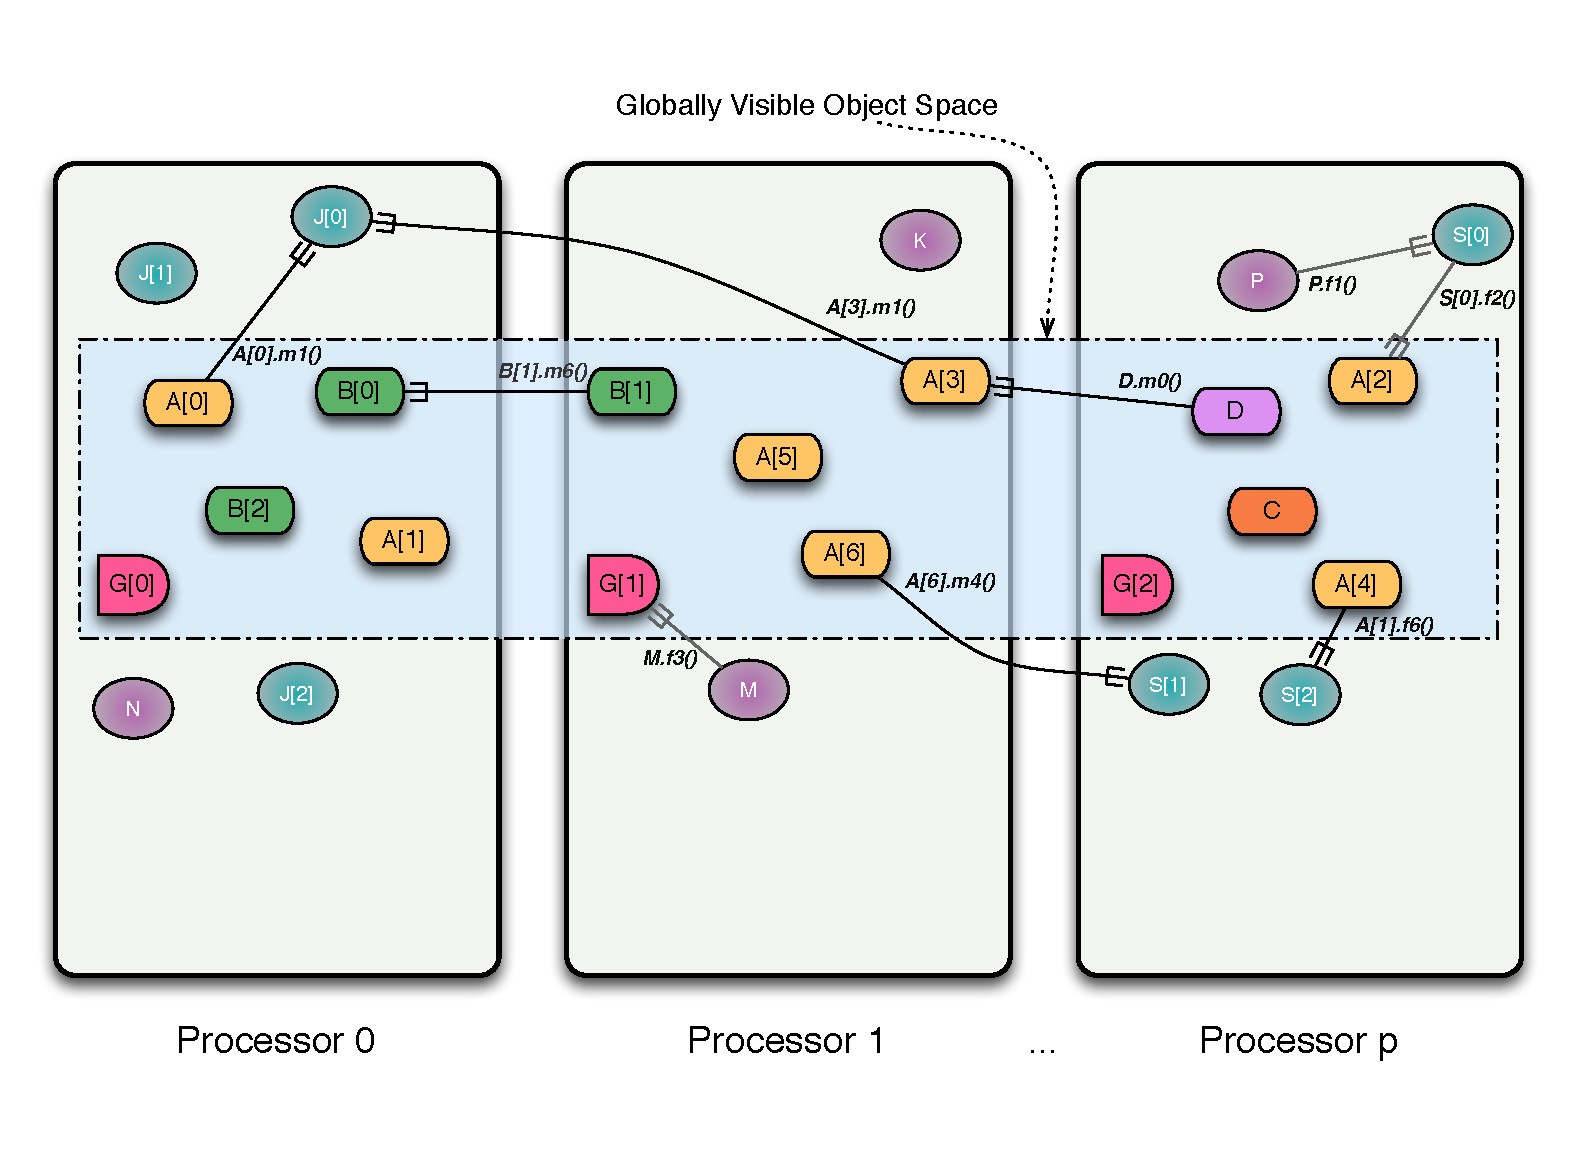
\includegraphics[width=0.9\textwidth]{../figures/progmodel/10-rmi-notgas.pdf}\end{figure}
\end{frame}


\begin{frame}
\frametitle{2. Not every method is remotely invocable}
%only subset of methods elevated into global namespace
%programmer annotates which methods are globally visible
%only globally visible methods can be invoked across proc boundaries
%intro term entry methods. will explain why later.
  \begin{figure}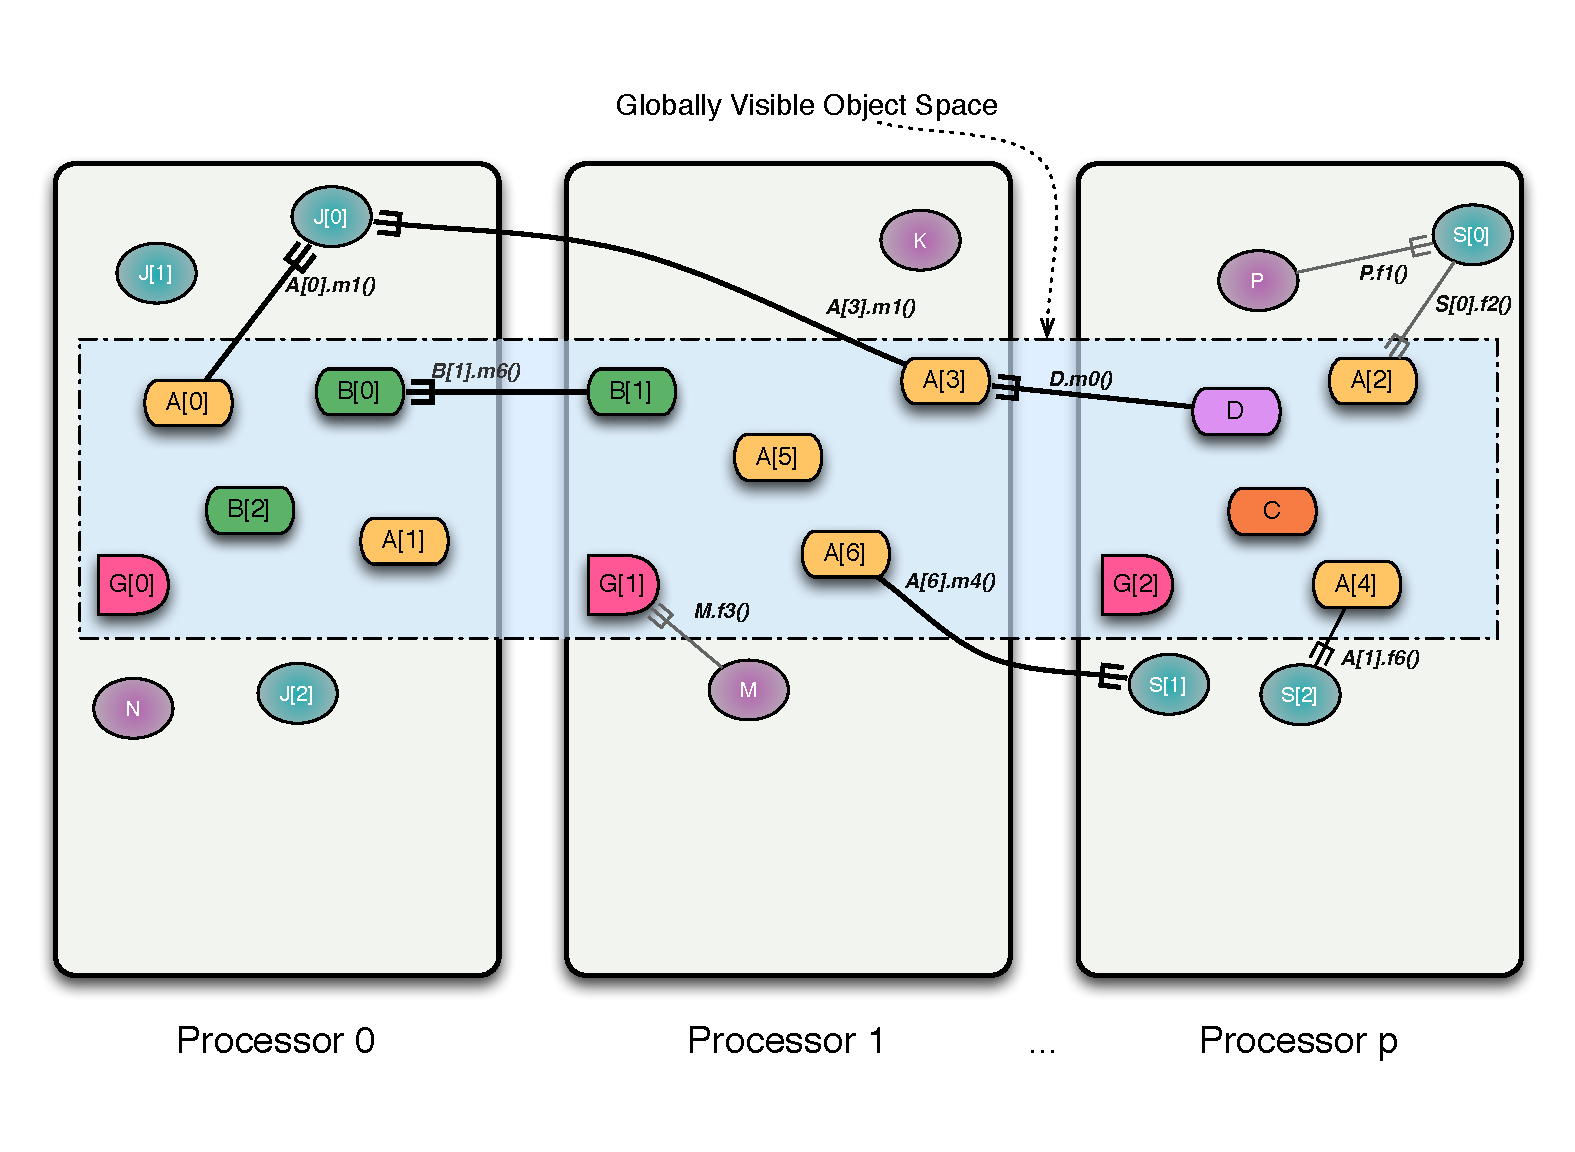
\includegraphics[width=0.9\textwidth]{../figures/progmodel/11-global-methods.pdf}\end{figure}
\end{frame}


\begin{frame}
\frametitle{3. Remote methods are of void return type}
  What happens if an object waits for a return value from a method invocation?
  \pause
  \begin{center}
    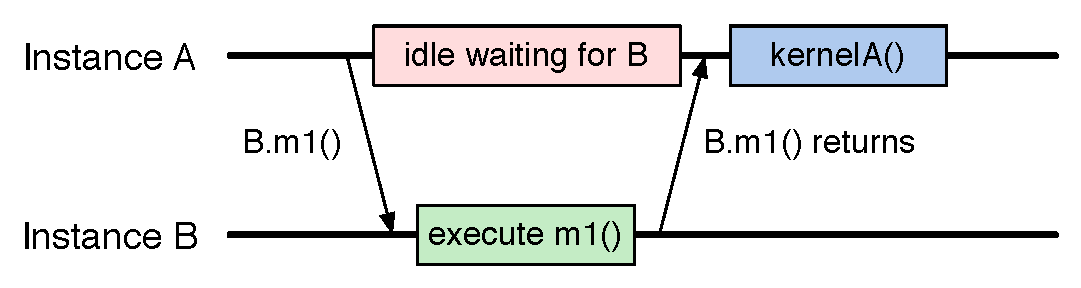
\includegraphics[width=\textwidth]{../figures/objectSequence.pdf}
  \end{center}
  \pause
  \begin{itemize}
    \item Performance
    \item Latency
    \item Reasoning about correctness
  \end{itemize}
\end{frame}


\begin{frame}
\frametitle{3. Remote methods are of void return type}
  \begin{center}
    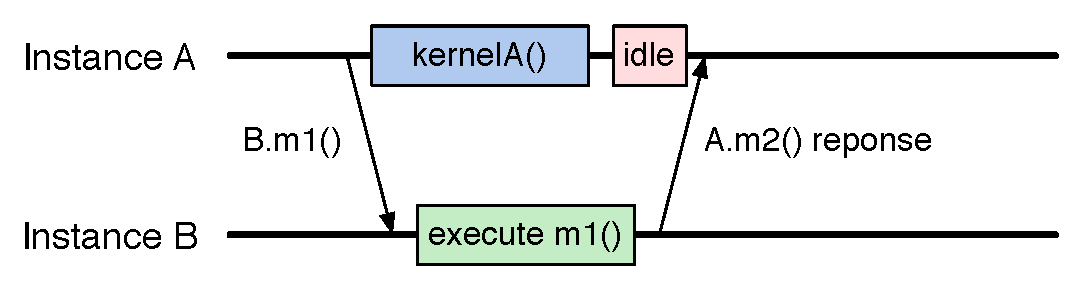
\includegraphics[width=\textwidth]{../figures/objectSequenceAsync.pdf}
  \end{center}
  \begin{itemize}
  \item Hence, method invocations should be asynchronous
    \begin{itemize}
    \item No return values
    \end{itemize}
  \item Computations are driven by the incoming data
    \begin{itemize}
    \item Initiated by the sender or method caller
    \end{itemize}
  \end{itemize}
\end{frame}


\begin{frame}
\frametitle{3. Remote methods are of void return type}
	Asynchronous, non-blocking remote method invocations
	\pause
	\begin{center}
        show fig with anchors removed from rmi, anchors on reg methods, and arrows too
        \includegraphics<1>[width=0.9\textwidth]{../figures/progmodel/11-global-methods.pdf}
        \includegraphics<2>[width=0.9\textwidth]{../figures/progmodel/12-asyn-nonblock-rmi.pdf}
	\end{center}
\end{frame}


\begin{frame}
\frametitle{How do you get return values}
	\begin{center}
        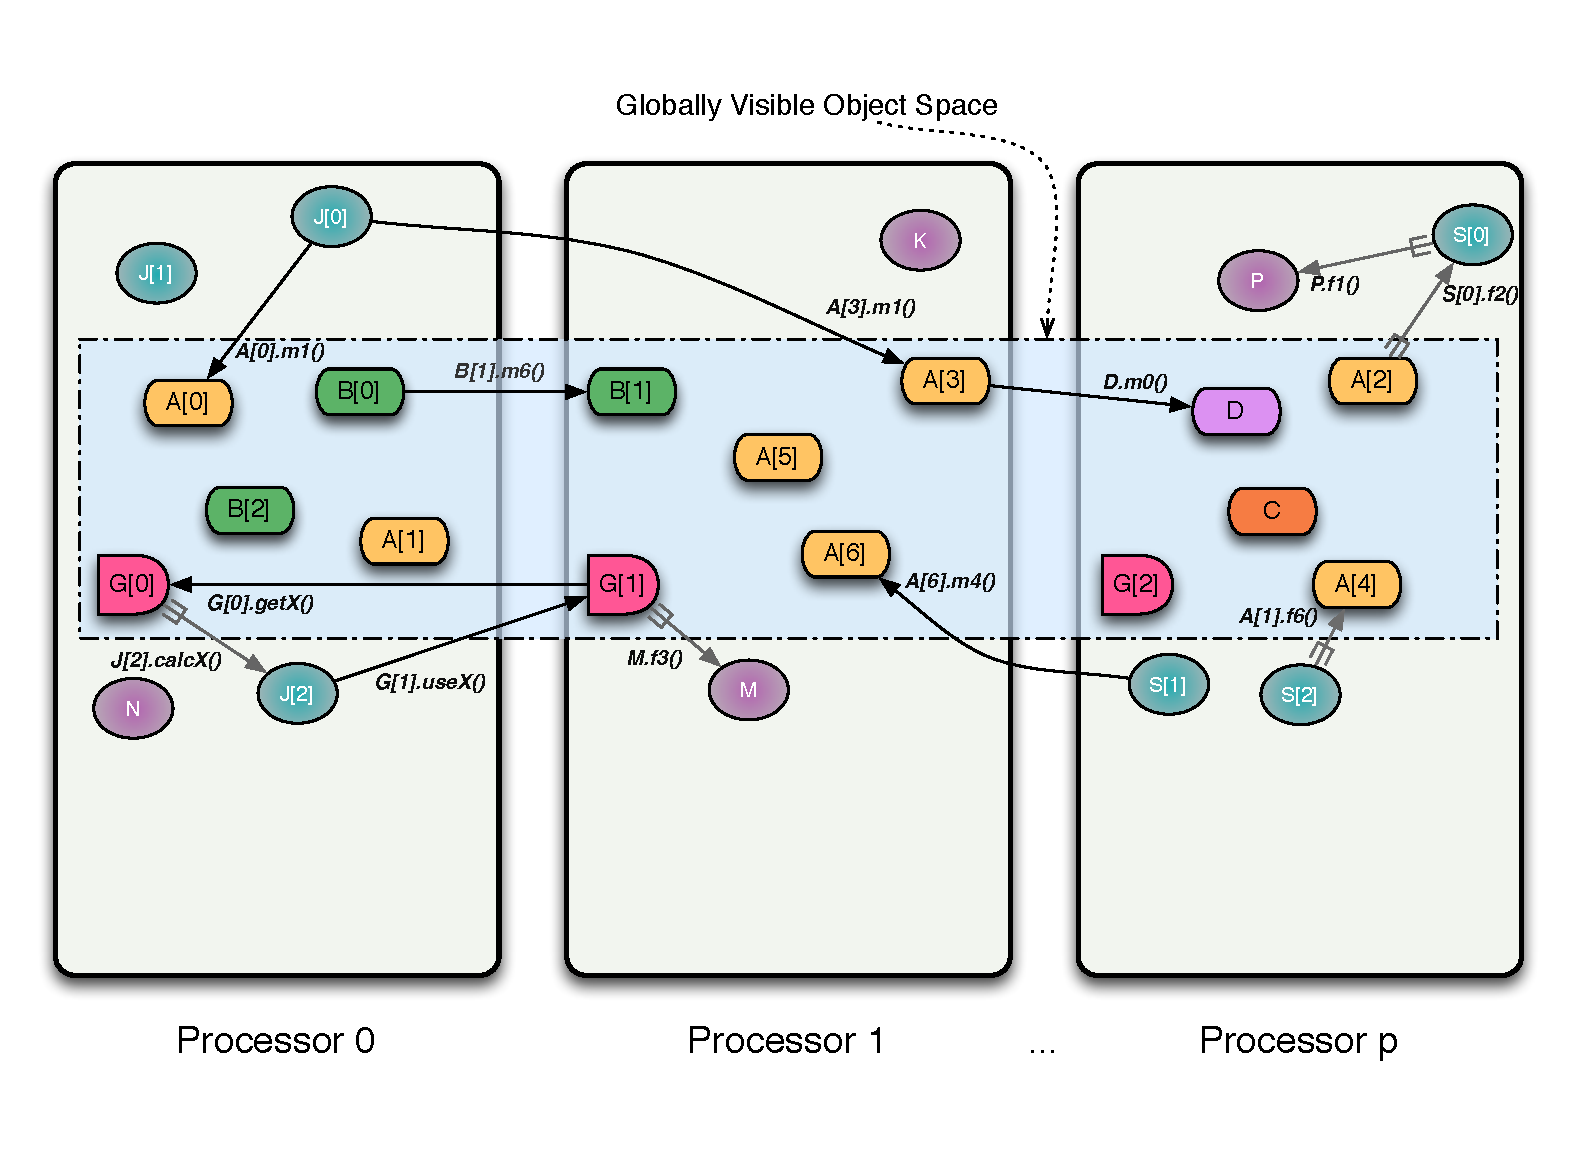
\includegraphics[width=0.9\textwidth]{../figures/progmodel/13-rmi-return-values.pdf}
	\end{center}
\end{frame}


\begin{frame}
\frametitle{Collective addressing}
	\begin{center}
        collective addressing (bcast, mcast)
        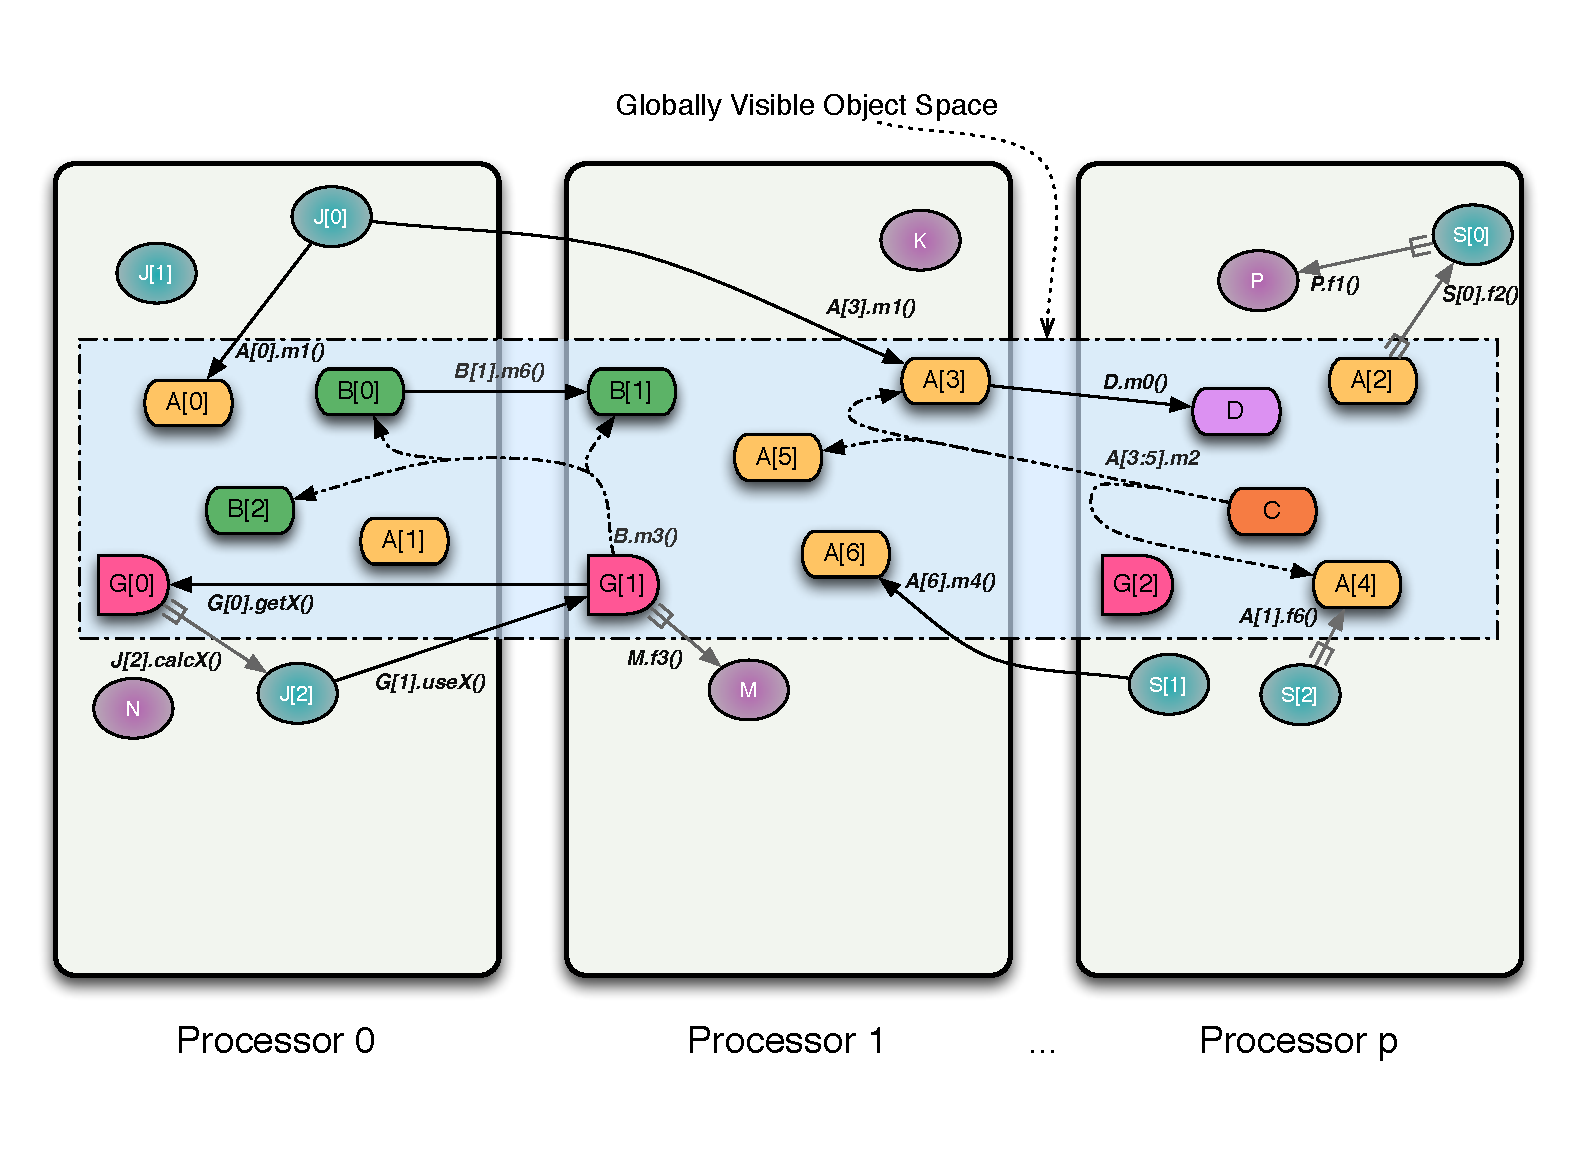
\includegraphics[width=0.9\textwidth]{../figures/progmodel/14-rmi-collective.pdf}
	\end{center}
\end{frame}


\begin{frame}
\frametitle{RMI expresses parallel dependencies}
	\begin{center}
        lu DAG?
        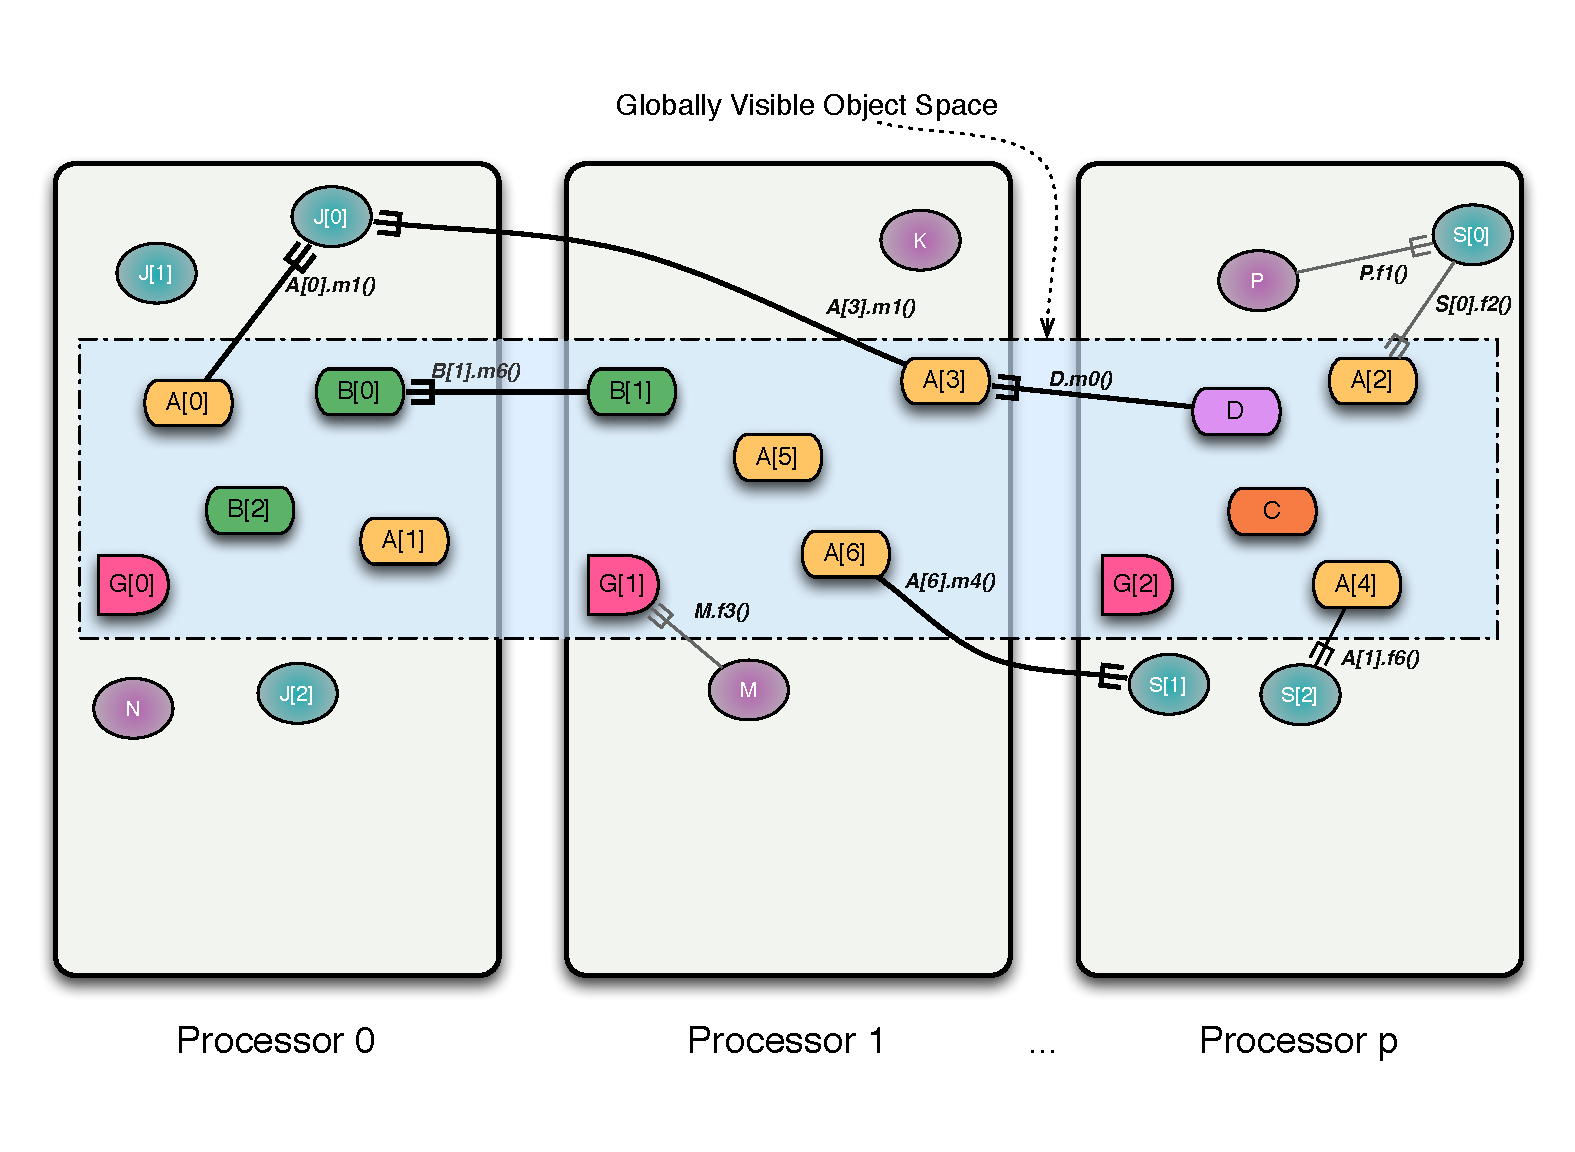
\includegraphics[width=0.9\textwidth]{../figures/progmodel/11-global-methods.pdf}
	\end{center}
\end{frame}



